\documentclass%
%[handout]
{beamer}
% % % % % % % %
% % % % % % % %
% % % % % % % %
%IMPORTANT
%compiles with 
%pdflatex -shell-escape 
%IMPORTANT
% % % % % % % %
% % % % % % % %
% % % % % % % %
\mode<presentation>
{
\useinnertheme{rounded}
\useoutertheme{infolines}
\usecolortheme{orchid}
\usecolortheme{whale}
}

\usepackage[english]{babel}
\usepackage[latin1]{inputenc}
\usepackage[all,cmtip]{xy}
\usepackage{times}
\usepackage[T1]{fontenc}
\usepackage{../example-templates}
\usepackage{../pstricks-commands}
\usepackage{cancel}

\usepackage{auto-pst-pdf}
\usepackage{pst-plot}
%\usepackage{pstricks-add} 

% Or whatever. Note that the encoding and the font should match. If T1
% does not look nice, try deleting the line with the fontenc.

\graphicspath{{../../modules/}}

\newtheoremstyle{partialproof}{3pt}{3pt}{}{}{}{.}{.5em}{}
\theoremstyle{partialproof} \newtheorem{partialproof}[theorem]{Proof.}
%\DeclareMathOperator{\diff}{d}
\newcommand{\diff}{\text{d}}
\setbeamertemplate{navigation symbols}{}

\includeonlylecture{1}

\newcommand{\lect}[3]{
  \date{#1}
  \lecture[#1]{#2}{#3}
}

\setbeamertemplate{footline}
{
  \leavevmode%
  \hbox{%
  \begin{beamercolorbox}[wd=.333333\paperwidth,ht=2.25ex,dp=1ex,center]{author in head/foot}%
    \usebeamerfont{author in head/foot}\insertshortauthor
  \end{beamercolorbox}%
  \begin{beamercolorbox}[wd=.333333\paperwidth,ht=2.25ex,dp=1ex,center]{title in head/foot}%
    \usebeamerfont{title in head/foot}\insertshorttitle
  \end{beamercolorbox}%
  \begin{beamercolorbox}[wd=.333333\paperwidth,ht=2.25ex,dp=1ex,center]{date in head/foot}%
    \usebeamerfont{date in head/foot}\insertshortdate{}
  \end{beamercolorbox}}%
  \vskip0pt%
}

% If you have a file called "university-logo-filename.xxx", where xxx
% is a graphic format that can be processed by latex or pdflatex,
% resp., then you can add a logo as follows:

%\pgfdeclareimage[height=0.8cm]{logo}{bluelogo}
%\logo{\pgfuseimage{logo}}

\begin{document}

\AtBeginLecture{%

\title[\insertlecture]{FreeCalc}
\subtitle{\insertlecture}
\author[FreeCalc]{}
\institute[UMass Boston]{University of Massachusetts Boston}
\date{\insertshortlecture}
\begin{frame}
  \titlepage
\end{frame}
}%

% begin lecture
\lect{\today}{Sample}{1}
%% begin module FTC-intro
\begin{frame}
\frametitle{(5.3) The Fundamental Theorem of Calculus}
\begin{itemize}
\item  The Fundamental Theorem of Calculus establishes a connection between differential calculus and integral calculus.
\item  It allows us to compute integrals very easily, without finding limits of Riemann sums.
\item  It has two different parts.
\item  Part 1 says, roughly, that ``differentiation undoes integration.''
\item  Part 2 says, roughly, that ``integration undoes differentiation.''
\item<2->  Part 1 deals with functions of the form
\[
\uncover<2->{%
g(x) = \int_a^x  f(t) \diff t%
}%
\]
\uncover<2->{where $f$ is a continuous function on $[a,b]$ and $x$ varies between $a$ and $b$.}
\end{itemize}
\end{frame}
% end module FTC-intro

%% begin module definite-integral-properties-split
\begin{frame}[t]
Properties of the Integral
\begin{enumerate}
\setcounter{enumi}{4}
\item  $\displaystyle %
\alertNoH{ 1}{\int_a^b f(x) \diff x} %
= %
\alertNoH{ 2}{\int_a^c f(x) \diff x} %
+ %
\alertNoH{ 3}{\int_c^b f(x) \diff x} %
$%
\end{enumerate}
\begin{center}
\psset{xunit=1.5cm, yunit=1.5cm}
\begin{pspicture}(-5, -5)(5,5)
\psframe*[linecolor=white](-5,-5)(5,5)
%Function formula: 1727/6250+4911/100 ((x)^{3})+110043/5000 (x)+3 ((x)^{5})-201/10 ((x)^{4})-52431/1000 ((x)^{2})
\uncover<1>{
\pscustom*[linecolor=\fcColorAreaUnderGraph]{
\psplot[linecolor=red, plotpoints=1000]{0.1}{2.5}{x 2 exp -52.431 mul x 4 exp -20.1 mul x 5 exp 3 mul x 22.0086 mul x 3 exp 49.11 mul 0.27632 add add add add add }
\psline(2.5, 0)(0.1,0)
}
}
\uncover<2>{
\pscustom*[linecolor=\fcColorAreaUnderGraph]{
\psplot[linecolor=red, plotpoints=1000]{0.1}{1.7}{x 2 exp -52.431 mul x 4 exp -20.1 mul x 5 exp 3 mul x 22.0086 mul x 3 exp 49.11 mul 0.27632 add add add add add }
\psline(1.7, 0)(0.1,0)
}
}
\uncover<3>{
\pscustom*[linecolor=\fcColorAreaUnderGraph]{
\psplot[linecolor=red, plotpoints=1000]{1.7}{2.5}{x 2 exp -52.431 mul x 4 exp -20.1 mul x 5 exp 3 mul x 22.0086 mul x 3 exp 49.11 mul 0.27632 add add add add add }
\psline(2.5, 0)(1.7,0)
}
}

\psline(0.1, 0.05)(0.1, -0.05)
\rput[t](0.1, -0.07){$a$}
\psline(1.7, 0.05)(1.7, -0.05)
\rput[t](1.7, -0.07){$c$}
\psline(2.5, 0.05)(2.5, -0.05)
\rput[t](2.5, -0.07){$b$}
\rput(1.5, 2.4 ){$y=f(x)$}
\psaxes[ticks=none, labels=none]{<->}(0,0)(-0.5,-0.5)(4.5,2.7)\tiny
\psplot[linecolor=red, plotpoints=1000]{0.1}{2.5}{x 2 exp -52.431 mul x 4 exp -20.1 mul x 5 exp 3 mul x 22.0086 mul x 3 exp 49.11 mul 0.27632 add add add add add }
\end{pspicture}
%\only<handout:0| -1>{%
%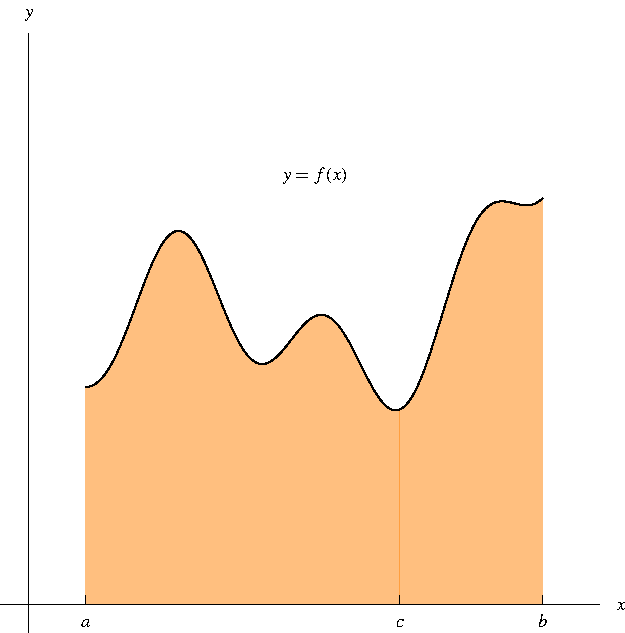
\includegraphics[height=5.6cm]{integration/pictures/05-02-splita.pdf}%
%}%
%\only<handout:0| 2>{%
%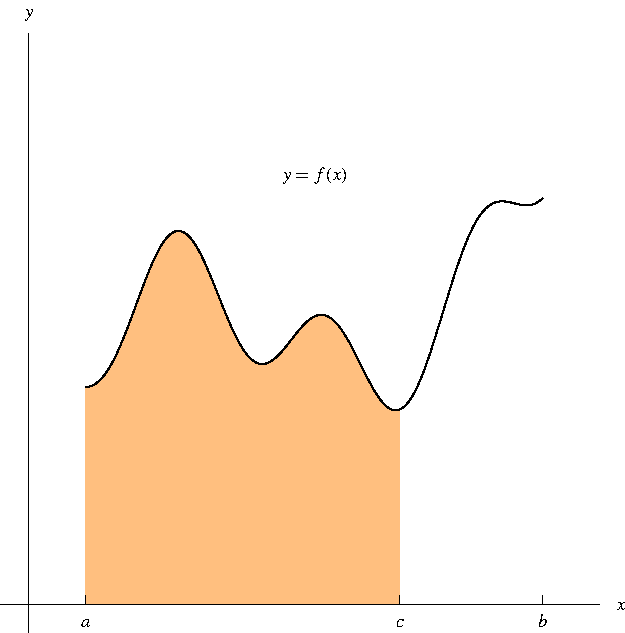
\includegraphics[height=5.6cm]{integration/pictures/05-02-splitb.pdf}%
%}%
%\only<handout:0| 3>{%
%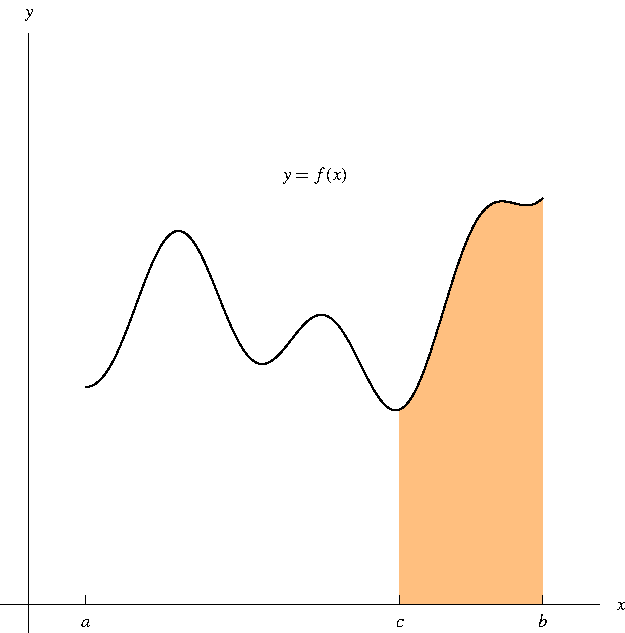
\includegraphics[height=5.6cm]{integration/pictures/05-02-splitc.pdf}%
%}%
\end{center}
\end{frame}
% end module definite-integral-properties-split

%% begin module definite-integral-properties-ex7
\begin{frame}
\begin{example}[Example 7, p. 352]
If it is known that \alert<handout:0| 5-6>{$\int_0^{10}f(x)\diff x = 17$} and \alert<handout:0| 7-8>{$\int_0^8 f(x) \diff x = 12$}, then find $\int_8^{10}f(x) \diff x$.
\abovedisplayskip=0pt
\belowdisplayskip=0pt
\abovedisplayshortskip=0pt
\belowdisplayshortskip=0pt
\begin{align*}
\uncover<2->{%
\int_{\alert<handout:0| 2-3>{0}}^{\alert<handout:0| 2-3>{8}} f(x)\diff x + \int_{\alert<handout:0| 2-3>{8}}^{\alert<handout:0| 2-3>{10}}f(x)\diff x%
}%
& \uncover<3->{ = } %
\uncover<3->{%
\int_{\alert<handout:0| 3>{0}}^{\alert<handout:0| 3>{10}}f(x)\diff x%
}\\%
\uncover<4->{%
\int_{\alert<handout:0| 2-3>{8}}^{\alert<handout:0| 2-3>{10}}f(x)\diff x%
}%
& \uncover<4->{ = } %
\uncover<4->{%
\alert<handout:0| 5-6>{\int_{\alert<handout:0| 3>{0}}^{\alert<handout:0| 3>{10}}f(x)\diff x} - \alert<handout:0| 7-8>{\int_{\alert<handout:0| 2-3>{0}}^{\alert<handout:0| 2-3>{8}} f(x)\diff x}%
}\\%
& \uncover<5->{ = } %
\uncover<5->{%
\alert<handout:0| 5-6>{\uncover<6->{17}} - \alert<handout:0| 7-8>{\uncover<8->{12}}%
}\\%
& \uncover<9->{ = } %
\uncover<9->{%
5%
}%
\end{align*}
\end{example}
\end{frame}
% end module definite-integral-properties-ex7

% WARNING: This next module could use some pictures.
%% begin module definite-integral-properties-comparison
\begin{frame}[t]
Comparison Properties of the Integral
\begin{enumerate}
\setcounter{enumi}{5}
\item  If $f(x)\geq 0$ for all $a\leq x \leq b$, then $\displaystyle \int_{a}^{b} f(x)\diff x \geq 0$.
\end{enumerate}
\end{frame}

\begin{frame}[t]
Comparison Properties of the Integral
\begin{enumerate}
\setcounter{enumi}{6}
\item  If $f(x)\leq g(x)$ for all $a\leq x \leq b$, then $\displaystyle \int_{a}^{b} f(x)\diff x \leq \int_{a}^{b} g(x)\diff x$.
\end{enumerate}
\begin{center}
\only<handout:0| -1>{%
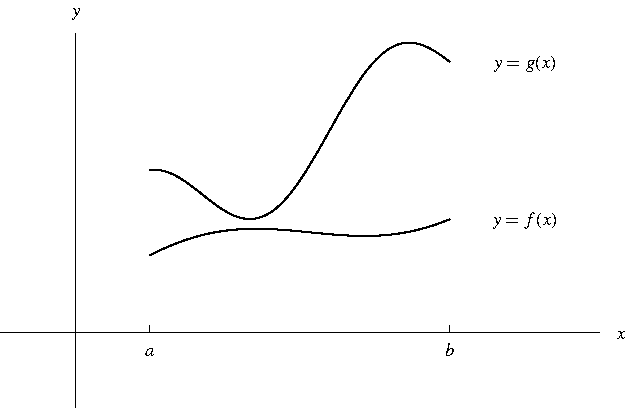
\includegraphics[height=4.2cm]{integration/pictures/05-02-comparisona.pdf}%
}%
\only<handout:0| 2>{%
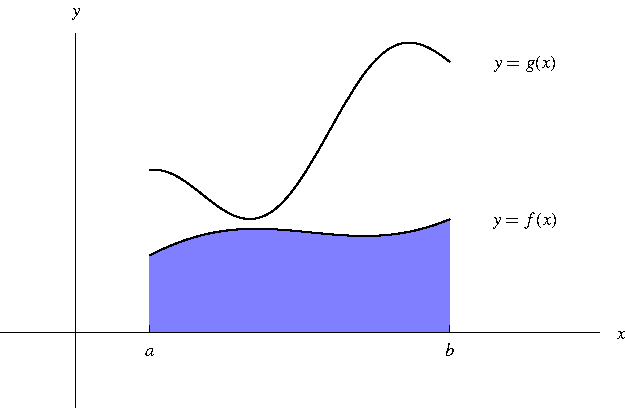
\includegraphics[height=4.2cm]{integration/pictures/05-02-comparisonb.pdf}%
}%
\only<handout:0| 3>{%
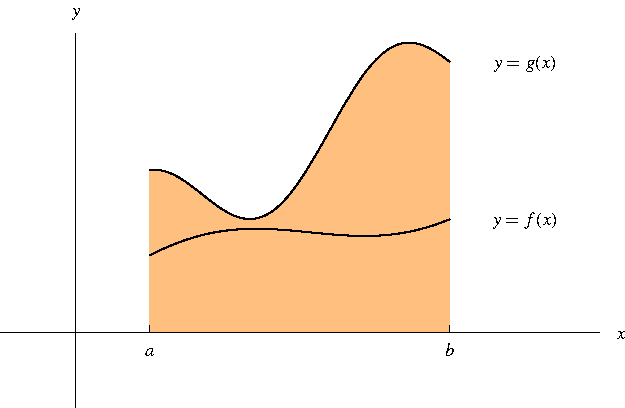
\includegraphics[height=4.2cm]{integration/pictures/05-02-comparisonc.pdf}%
}%

\[
\alert<handout:0| 2>{\int_a^b f(x) \diff x}%
 \leq  %
\alert<handout:0| 3>{\int_a^b g(x) \diff x}%
\]
\end{center}
\end{frame}

\begin{frame}[t]
Comparison Properties of the Integral
\begin{enumerate}
\setcounter{enumi}{7}
\item  If $m\leq f(x)\leq M$ for all $a\leq x \leq b$, then 
\[
\alert<handout:0| 2>{m(b-a)}%
 \leq  %
\alert<handout:0| 3>{\int_a^b f(x) \diff x}%
 \leq  %
\alert<handout:0| 4>{M(b-a)}%
\]
\end{enumerate}
\begin{center}
\only<handout:0| -1>{%
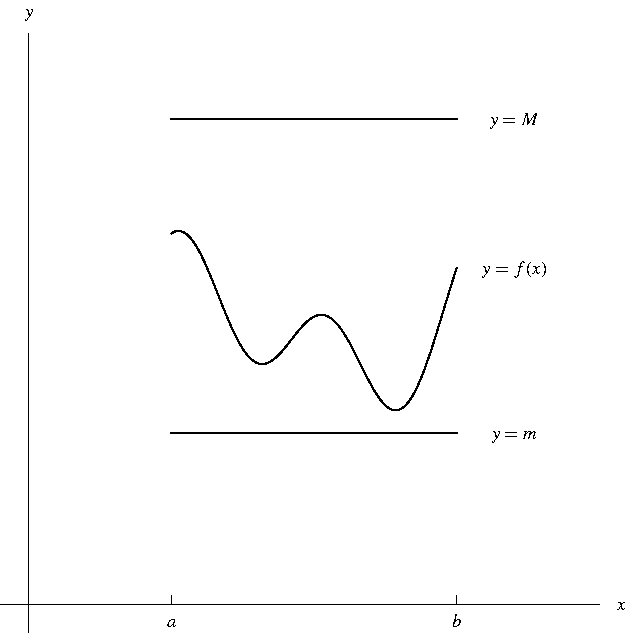
\includegraphics[height=5.6cm]{integration/pictures/05-02-boundinga.pdf}%
}%
\only<handout:0| 2>{%
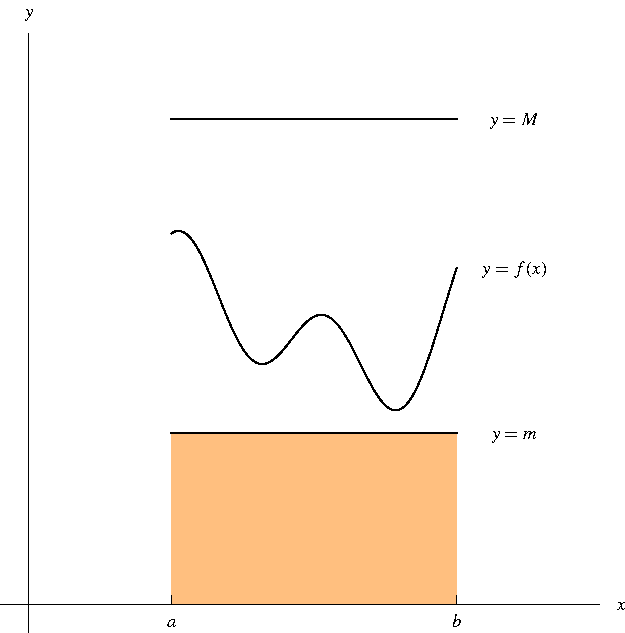
\includegraphics[height=5.6cm]{integration/pictures/05-02-boundingb.pdf}%
}%
\only<handout:0| 3>{%
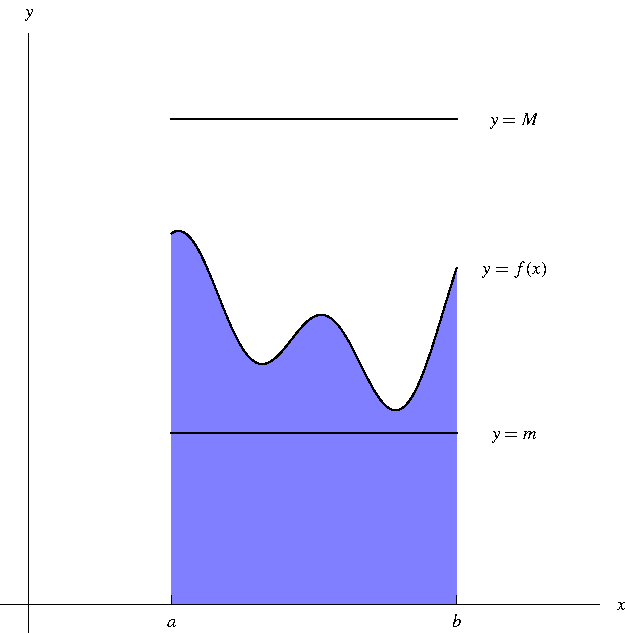
\includegraphics[height=5.6cm]{integration/pictures/05-02-boundingc.pdf}%
}%
\only<handout:0| 4>{%
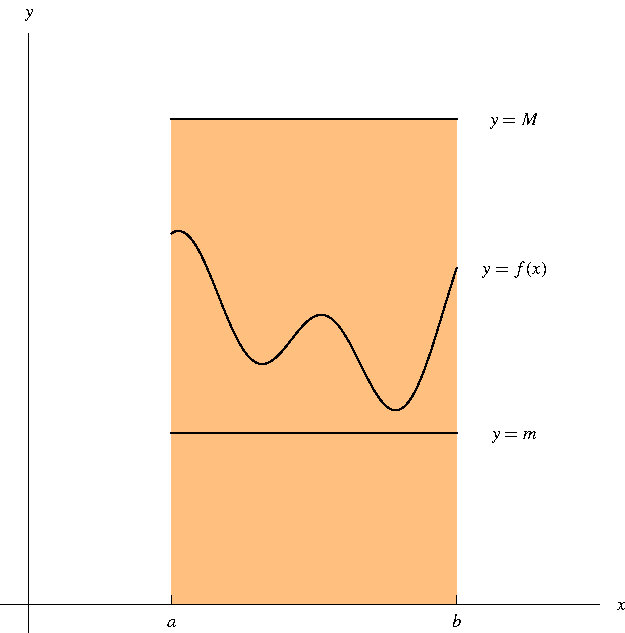
\includegraphics[height=5.6cm]{integration/pictures/05-02-boundingd.pdf}%
}%
\end{center}
\end{frame}
% end module definite-integral-properties-comparison

% begin module FTC-part2-ex7
\begin{frame}
\begin{example} %[Example 2, p. 357]
\begin{columns}
\column{0.4\textwidth}
\psset{xunit=0.7cm, yunit=0.7cm}
\begin{pspicture}(-1.000000, -1.3)(6.2,1.3)
\tiny
\psframe*[linecolor=white](-1.000000,-1.1)(6.2,1.2)
\pscustom*[linecolor=cyan]{ %Function formula: \cos{}x
\psplot[linecolor=\fcColorGraph, plotpoints=1000]{0}{1}{x 57.29578 mul cos }\psline(1.000000, 0)(0.000000, 0)}
%Function formula: \cos{}x
\psplot[linecolor=\fcColorGraph, plotpoints=1000]{0}{6}{x 57.29578 mul cos }
\psaxes[arrows=<->, ticks=none, labels=none](0,0)(-0.6,-1.1)(6,1.1)
\fcLabels{6}{1.1}
\fcXTickWithLabel{1}{$b$}
\end{pspicture}
\column{0.6\textwidth}
Find the area under the cosine curve from $0$ to $b$, where $0 \leq b \leq \frac{\pi}{2}$.
\end{columns}
\begin{itemize}
\item<2->  $\cos x$ is continuous on $[0, \frac{\pi}{2}]$ (in fact, it's continuous everywhere).
\item<3-| alert@3-4>  An antiderivative is \uncover<4->{$\sin x$.}
\[
\uncover<5->{%
\int_{\alert<handout:0| 5>{0}}^{\alert<handout:0| 5>{b}} \cos x \ \diff x = \left[ \sin x \right]_{\alert<handout:0| 5>{0}}^{\alert<handout:0| 5>{b}} %
}%
\uncover<6->{%
 = \sin (b) - \sin (0)%
}%
\uncover<7->{%
 = \sin b%
}%
\]
\end{itemize}
\end{example}
\end{frame}
% end module FTC-part2-ex7


%% begin module FTC1-proof
\begin{frame}
\begin{theorem}[The Fundamental Theorem of Calculus part 1]
Let \alert<2>{$f$ be a function continuous on $[a, b]$} and let $G(x) = \displaystyle \int_a^x f(t) \diff t$ for all $x\in [a,b]$. Then $G$ is differentiable and $G'(x) = f(x)$.  
\end{theorem}
\begin{proof}[Proof]
\begin{columns}
\column{0.27\textwidth}
\psset{xunit=0.9cm, yunit=0.9cm}

\begin{pspicture}(-0.5, -5)(2.5,5) 
\psframe*[linecolor=white](-0.5,-5)(5,5) 
\tiny 
%\psLabels{3}{2.5}

\pscustom*[linecolor=cyan]{
\psplot[linecolor=\psColorGraph, plotpoints=1000]{0.5}{2}{1 -0.5 x add 3 exp 0.333333 mul add -0.5 x add 2 exp -0.5 mul add }
\psline(2,0)(0.5,0) 
}
\uncover<20,21>{
\pscustom*[linecolor=red]{
\psplot[linecolor=\psColorGraph, plotpoints=1000]{0.5}{2}{1 -0.5 x add 3 exp 0.333333 mul add -0.5 x add 2 exp -0.5 mul add }
\psline(2,0)(0.5,0) 
}
}

\uncover<11->{
\pscustom*[linecolor=blue]{
\psplot[linecolor=\psColorGraph, plotpoints=1000]{2}{2.15}{1 -0.5 x add 3 exp 0.333333 mul add -0.5 x add 2 exp -0.5 mul add }
\psline(2.15,1.136125)(2.15,0)(2,0)
}
}

\uncover<10,20,22>{
\pscustom*[linecolor=red]{
\psplot[linecolor=\psColorGraph, plotpoints=1000]{2}{2.15}{1 -0.5 x add 3 exp 0.333333 mul add -0.5 x add 2 exp -0.5 mul add }
\psline(2.15,1.136125)(2.15,0)(2,0)
}
}

\uncover<12>{
\pscustom*[linecolor=red]{
\psplot[linecolor=\psColorGraph, plotpoints=1000]{2}{2.15}{1 -0.5 x add 3 exp 0.333333 mul add -0.5 x add 2 exp -0.5 mul add }
\psline(2.15,1.136125)(2.15,1)(2,1)
}
}

\psaxes[ticks=none, labels=none]{<->}(0,0)(-0.5,-0.5)(3.2,3.083333)

%Function formula: -1/2 (x-1/2)^{2}+1/3 (x-1/2)^{3}+1 
\psplot[linecolor=\psColorGraph, plotpoints=1000]{0.5}{3}{1 -0.5 x add 3 exp 0.333333 mul add -0.5 x add 2 exp -0.5 mul add }
\rput[b](2.3, 2.4){$y=f(x)$}
\uncover<11,14>{
\psline*[linecolor=red](2,0)(2.15,0)(2.15,1)(2,1)(2,0)
}
\uncover<13->{
\psline(2,0)(2.15,0)(2.15,1.136125)(2,1.136125)(2,0)
}

\psXTick{2} 

\uncover<3>{ %
\psline[linecolor=red, linewidth=2pt](1.5,0)( 2.5,0 )
}
\uncover<4-7>{ %
\psline[linewidth=2pt](1.5,0)( 2.5,0 )
}

\uncover<4>{ %
\psline[linecolor=red, linewidth=2pt](2,0)(2,1)
}

\uncover<6>{ %
\psline(2.4,1.481333)(2.4,0)
}
\uncover<5>{ %
\psline[linecolor=red, linewidth=2pt](2.4,0)(2.4,1.481333)
}

\uncover<5-7>{ %
\psline(2,0)(2,1)
}
\uncover<5>{ %
\psline[linecolor=red](2.4,0)(2.4,1.481333)
}
\uncover<6>{ %
\psline[linecolor=red, linewidth=2pt](2,1)(2, 1.481333)
}
\psXTickWithLabel{0.5}{$a$}

\psXTick{3}
\rput[tl](3,-0.2){$b$}
\uncover<7->{
\psXTick{2.15}
\rput[tl](2.15, -0.2){$x+h$}
}
\uncover<7,13>{
\psline[linecolor=red, linewidth=2pt](2,0)(2.15,0)
}
\rput[tr](2, -0.235){$x$}
\end{pspicture}

\vspace{1.68cm}
\column{0.73\textwidth}

\only<1-15>{
\uncover<2->{\alert<2>{Let $\varepsilon >0$. There \alert<3>{exists $\delta$} such that $\alert<8>{\alert<6>{|\alert<5>{f(t)}-\alert<4>{f(x)}|} < \varepsilon}$ for all $t$ for which $|x-t|<\delta$}.} \uncover<3->{\alert<7>{Then for all $0<h<\delta$:} }
\[
\begin{array}{rlll|l}
\uncover<8->{\alert<8>{\varepsilon} &\alert<8>{ > \hphantom{ \int_{ x}^{ x+h}(} f(t)-f(x) } & \alert<8>{ > - \varepsilon }  &\uncover<9->{&\text{integrate}} }\\
\uncover<9->{h\varepsilon  & >\alert<12>{ \alert<10,11>{\int_{x }^{x+h}} ( \alert<10>{ f(t)}-\alert<11>{f(x)})\alert<10,11>{ dt} }&>-h\varepsilon &\uncover<13->{& \text{divide~by~}\alert<13>{h }} } \\
\uncover<13->{\varepsilon& >\frac{\alert<14>{\int_{x }^{x+h}}(f(t) -\alert<14>{f(x)}) \alert<14>{dt}}{ \alert<13,14>{ h} }& >-\varepsilon}\\
\uncover<14->{\alert<15>{\varepsilon}&\alert<15>{>} \frac{\int_{x }^{x+h}f(t)dt }{h}- \alert<14>{\frac{h f(x)}{h}} &\alert<15>{ > - \varepsilon}}\\
\uncover<15->{\varepsilon&\color{red} >  \left| \color{black} \frac{\int_{x }^{x+h}f(t)dt }{h} - f(x)\color{red} \right|}\\
\end{array}
\]
}

\only<16->{
\uncover<17->{In analogous fashion  \alert<17>{we can handlethe case $h<0$}, to prove:} \alert<23>{ for any $\varepsilon >0$ there exists $\delta>0$ so that for \\ all $\only<16>{0<h\phantom{|}} \alert<17>{\only<17->{\phantom{0<}|h|}} \alert<17>{<\delta}$ we have $\left| \frac{\int_{x }^{x+h}f(t)dt }{h}-f(x)\right|<\varepsilon$.}

\[
\begin{array}{l}
\uncover<18->{\displaystyle G'(x)=\lim\limits_{h\to 0}\frac{ \alert<20>{ G(x+h)} -\alert<21>{G(x)}}{h} }\\ 
\uncover<19->{\displaystyle \phantom{ G'(x) }= \lim\limits_{h\to 0}  \frac{ \alert<20>{ \alert<22>{\int_{a}^{x+h}} f(t)dt} - \alert<21>{ \alert<22>{\int_{a}^{x}} f(t)dt}}{h} }\\
\uncover<22->{\displaystyle \phantom{ G'(x) }= \alert<23>{\lim\limits_{h\to 0}\frac{\alert<22>{\int_{x}^{x+h}}f(t)dt }{h} \uncover<23->{=f(x)}}}
\end{array}
\]

}
\end{columns}
\end{proof} 
\end{frame}
% end module FTC1-proof


\end{document}
